\begin{definition}[Inforamtion Set]
    An \textbf{information set} is a collection of histories with the the property that the player who is going to move, doesn't know which history has been reached given that one of these histories was reached.
\end{definition}


\begin{definition}[information Partition]
    An \textbf{information partition} is a collection of information sets.
\end{definition}


\begin{example}
    Assume that after player $i$ moves $H_i = \{C,D,E\}$
    \begin{enumerate}[label=P\arabic*:]
        \item $\{C\}, \{D,E\}$: player knows whether C occurred or not
        \item $\{C\}, \{D\}, \{E\}$: player knows whether C, D or E occurred
        \item $\{C,D,E\}$: player does not know whether C, D or E occurred
    \end{enumerate}
\end{example}

\begin{remark}
    Any strategic game can be presented as an extensive game with imperfect information.
\end{remark}

\begin{example}[Battle of Sexes]
    In the Battle of Sexes, player 2 does not know wether she is on the left or right side of the tree. This is denoted by the red line with `2'. In any information set, it must be the case that the player is choosing between the same actions. If this is not the case, the property (unknown history) from an information set is not longer true.

    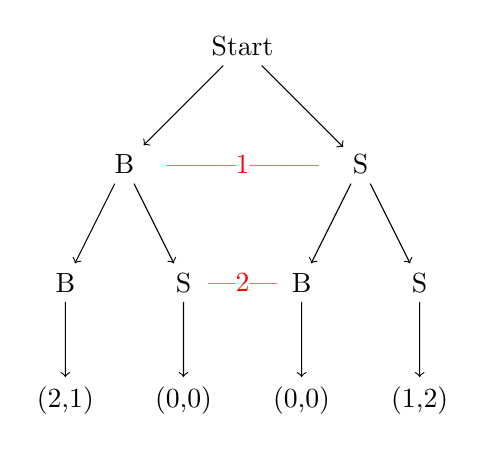
\begin{tikzpicture}[->]
        \node {Start}
        child { node {B}
                child { node {B} child {node{(2,1)}}}
                child { node {S} child {node{(0,0)}}}
            }
        child[color=white] { node[color=red,] {--------1--------} child {node[color=red] {---2---}}}
        child { node {S}
                child { node {B} child {node{(0,0)}}}
                child { node {S} child {node{(1,2)}}}
            };
    \end{tikzpicture}
\end{example}


\begin{illustration}[Definition extensive game/application to BoS]Formally, a extensive game has the following form:
    \begin{itemize}[noitemsep]
        \item Players
              \begin{itemize}[noitemsep]
                  \item Player 1
                  \item Player 2
              \end{itemize}
        \item Terminal histories
              \begin{itemize}[noitemsep]
                  \item (B,B)
                  \item (B,S)
                  \item (S,B)
                  \item(S,S)
              \end{itemize}
        \item Player function
              \begin{itemize}[noitemsep]
                  \item $P(\varnothing)=1$
                  \item $P(B)=2$
                  \item $P(S)=2$
              \end{itemize}
        \item Chance moves: none
        \item Information partitions:
              \begin{itemize}[noitemsep]
                  \item Player 1: $\varnothing$
                  \item Player 2: $\{B,S\}$
              \end{itemize}
        \item Preferences: as given in the graph above.
    \end{itemize}
\end{illustration}

\begin{illustration}[Card game] Our Card game is played as follows:
    \begin{itemize}
        \item Player 1 and player 2 put \$1 in the pot.
        \item A card is drawn.
        \item Player 1 is informed whether card is `high' or `low', player 2 is not informed.
        \item Player 1 can choose between (`see' and `raise')
              \begin{itemize}
                  \item If Player 1 chooses `see', then the game is finished. The card determines who wins dollar. `high' means player 1 gets the money, `low' means player 2 gets the money.
                  \item If player 1 chooses `raise', then she adds \$1 to the pot. Then Player 2 can choose (`pass' or `meet')
                        \begin{itemize}
                            \item If player 2 chooses `pass', player 1 takes the money.
                            \item If player 2 chooses `meet', she adds \$1 to pot.
                        \end{itemize}
              \end{itemize}
    \end{itemize}
\end{illustration}


\begin{illustration}[Nash Equilibrium of Card game] To find the Nash Equilibrium of the Card Game, write down the game in strategic form. In this table, (Raise, See) denotes player 1’s strategy to Raise after High and See after Low.

    \begin{table}[h!]
        \begin{center}
            \begin{tabular}{ c | c c c c}
                             & Pass   & Meet                           & \\ \hline
                Raise, Raise & (1,-1) & (0,0)                            \\
                Raise, See   & (0,0)  & ($\frac{1}{2}$,$-\frac{1}{2}$)   \\
                See, Raise   & (1,-1) & ($-\frac{1}{2}$,$\frac{1}{2}$)   \\
                Raise, Raise & (0,0)  & (0,0)
            \end{tabular}
            \caption{Strategic form of Card game}
        \end{center}
    \end{table}
    We can conclude that there are no pure strategies Nash equilibrium. Furthermore, (See, See) is strictly dominated by ($\frac{1}{2}$, Raise Raise; $\frac{1}{2}$, Raise See). This means (See, See) is not played in any Nash equilibrium.
    We also see that (See, Raise) is weakly dominated by (Raise, Raise). Given that $q=1$ (probability 1 to pass) cannot be part of Nash equilibrium, (See, Raise) is not used in any Nash equilibrium. We can now reduce our table.

    \begin{table}[h!]
        \begin{center}
            \begin{tabular}{ c c c c c}
                           & Pass   & Meet                           &      \\ \hline
                Raise, See & (0,0)  & ($\frac{1}{2}$,$-\frac{1}{2}$) & p    \\
                See, Raise & (1,-1) & ($-\frac{1}{2}$,$\frac{1}{2}$) & 1 -p \\
                           & q      & 1-q
            \end{tabular}
            \caption{Reduced Strategic form of Card game with probabilities}
        \end{center}
    \end{table}

    There are mixed strategies Nash equilibria in the remaining game. We have row-player indifferent if $q = (1/2)(1-q)$, thus $q = 1/3$. We also have column-player indifferent if: $-p = -(1/2)(1-p)$, thus $p = 1/3$.

    So, unique Nash equilibrium:
    player 1 assigns 1/3 to (Raise, Raise); 2/3 to (Raise, See) and
    player 2 assigns 1/3 to pass; 2/3 to meet

    In words, this means player 1 will always chooses `raise' after `high' and bluffs after `low' with probability 1/3

    This means that Card Game is favorable to player 1. You should refuse the role of player 2 if you can.
\end{illustration}


\begin{illustration}[Repated games: prisoner's dilemma] The main idea of this game is to sustain cooperation in equilibrium by threatening to switch to punishment if the other does not cooperate.

    \begin{table}[h!]
        \begin{center}
            \begin{tabular}{ c | c c c c}
                  & C     & D     & \\ \hline
                C & (2,2) & (0,3)   \\
                D & (3,0) & (1,1)
            \end{tabular}
            \caption{Payoff matrix for the prisoner's dilemma}
        \end{center}
    \end{table}

    There are two strategies:\\
    \textbf{Grim trigger strategy}
    \begin{itemize}
        \item start with C
        \item continue with C as long as other player chooses C
        \item if in any period other chooses D, then choose D in every subsequent period
    \end{itemize}
    \textbf{Tit-for-tat}
    \begin{itemize}
        \item start with C
        \item do whatever the other player did in previous period
    \end{itemize}
    We have some notation. Player $i$ uses discount factor $\delta$ for which $0 < \delta < 1$
    $$
        u_i(a^{1}, a^{2}, \ldots, a^{{T}}) = u_i(a^{1})+\delta u_i(a^{2})+\delta^{2} u_i(a^{3})+\ldots+\delta^{{T}-1} u_i(a^{{T}})
        =\sum_{t=1}^{T} \delta^{t-1} u_i(a^{t})
    $$
    There is a possibility that $T \to \infty$. Or that there is a $p$: a probability the game is finished at a given period.
\end{illustration}

\begin{example}
    Let $c$ be the value that makes player indifferent between payoffs $c, c, c, ... $ and payoffs
    $w^1 , w^2 , w^3 , ...$.
    Let $V$ denote the value of discounted sum $w^1 , w^2 , w^3 , ...$. We can find this $c$ as follows:
    \begin{align*}
        V =           & c + c\delta + c\delta^2 + c\delta^3 + ... \\
        V\delta =     & c\delta + c\delta^2 + c\delta^3 + ...     \\
        V-\delta V =  & c \tag{subtract \delta V from both sides} \\
        (1-\delta)V = & c
    \end{align*}
    So discounted average $c$ equals $(1 - \delta)V$
\end{example}

\begin{remark}
    A repeated game is an extensive game with perfect information and
    simultaneous moves. This mean we can use concept of subgame perfection. If the game is finitely repeated $n$ times, we can apply backwards induction (starting at the $n$th period).
\end{remark}

\begin{example}[Finitely repeated Prisoner's dilemma]
    Unique subgame perfect equilibrium: each player's strategy chooses D in every period (proof by backward induction). In any finitely repeated game every Nash equilibrium generates outcome (D,D) in every period. To support cooperation in equilibrium, it is required that the game is infinitely repeated.
\end{example}


\begin{illustration}
    Some Nash equilibria of infinitely repeated PD
    \begin{enumerate}

        \item Every player always plays D whatever happened
        \item Grim trigger strategy is N.E. if $\delta$ is sufficiently large. Assume other player plays grim trigger and that layer $i$ considers to deviate to D in period k. The discounted average deviation from period $k$ equals
              $(1-\delta)(3+\delta+\delta 2 +\delta 3 +...)=(1-\delta)(3+\delta/(1-\delta))=3(1-\delta)+ \delta$
              discounted average if $i$ sticks to grim trigger $ = 2$
              In conclusion, Grim trigger is a best response if
              $$2 > 3(1-\delta)+ \delta \iff \delta > 1/2$$
        \item  Tit-for-tat
              Assume other player plays tit-for-tat
              and that player $i$ considers to deviate to D in period $k$
              \begin{enumerate}


                  \item Player $i$ reverts to $C$ in period $k+1$. If this is part of her best response, she should continue alternating (situation is stationary). The discounted average payoff alternating from period $k$:
                        \[(1-\delta)(3+0\delta+3\delta 2 +0\delta 3 +3\delta 4 +...)=3(1-\delta)/(1-\delta 2 )=3/(1+\delta)
                        \]
                        Alternating does not beat tit-for-tat if
                        \[
                            3/(1+\delta) < 2 \iff \delta > 1/2
                        \]

                  \item player $i$ sticks to D after $k$. Then she earns
                        $$(1-\delta)(3+\delta+\delta 2 +\delta 3 +...=(1-\delta)(3+\delta/(1-\delta))=
                            3(1-\delta)+ \delta \le 2 \iff \delta \ge 1/2$$
              \end{enumerate}
    \end{enumerate}

    But many more outcomes can be supported in equilibrium of the infinitely repeated prisoner's dilemma.
\end{illustration}

\begin{theorem}[Folk Theorem]
    \begin{itemize}
        \item For any discount factor $\delta$ with $0<\delta<1$, the discounted average payoff of any player $i$ in any Nash equilibrium is at least $u_i (D,D)$.
        \item Let $(x_1 ,x_2)$ be a feasible pair of payoffs such that $x_i >u_i (D,D)$ for each $i$. There exists a
              $\delta^* \le 1$ such that if $\delta>\delta^* $, then the game has a N.E. in which the discounted payoff of each
              player $i$ is $x i$ .
        \item For any $\delta$ the game has a N.E. in which the average discounted payoff of player $i$ equals $u_i (D,D)$
    \end{itemize}
\end{theorem}
\begin{proof}

\end{proof}
\begin{illustration}[Nash equilibria of infinitely repeated PD with mistakes]
    What about environments where players may make mistakes? grim trigger does not do so well, tit-for-tat works better. But, the winner is Pavlov strategy
    ("win-stay lose-change"):
    \begin{itemize}
        \item Start with C
        \item Choose C if previous outcome was (C,C) or (D,D)
        \item Choose D after any other history
    \end{itemize}
\end{illustration}

